%!TEX root = ../thesis.tex
\section{Simple Contract Net}

In this scenario, one agent sends a call for proposals (CFP) to multiple agents which then reply with their individual proposals. This simple scenario was created to test the core of SAJaS and the plugin. The goal was not only to create a working simulation model based on SAJaS, but also to demonstrate that the execution of a simulation in SAJaS and the equivalent JADE application generated from it are identical and that performance in SAJaS is higher.

\subsection{Experimental Setup}

The diagram in Figure \ref{fig:CNetExample} illustrates the contract net created for this test. An agent (the buyer) intends to purchase a certain quantity of three kinds of goods: rice, flour and oats. Besides the quantities of each product it needs, the buyer also stipulates a maximum price for the whole deal. The buyer will issue a call for proposals (CFP) containing a request for supplies to all agents that announce themselves as suppliers in the DF.

Supplier agents have a maximum supply capacity and a price for each product. After receiving a CFP, the supplier replies with a PROPOSAL containing a price for each product if the demanded supply is within the seller's capacity. Otherwise, a REFUSE message will be sent to the buyer.
Finally, the buyer agent compares all valid proposals, chooses the cheapest offer for each of the three products and replies with an ACCEPT PROPOSAL to the best offers, and REJECT PROPOSAL to all others.

\begin{figure}[h]
	\centering
	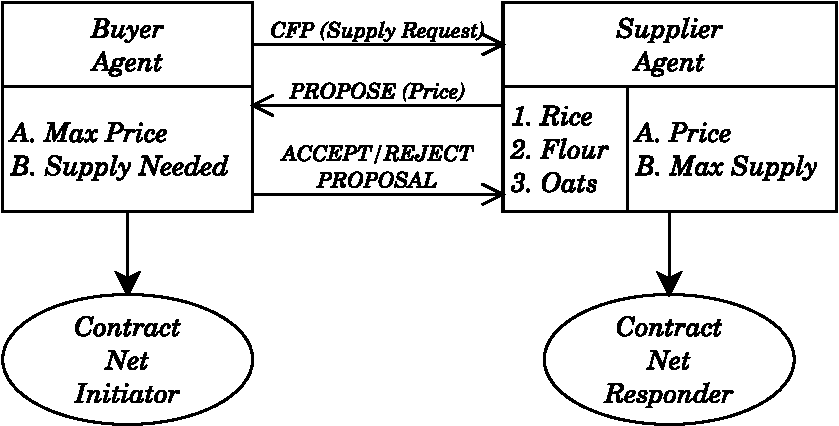
\includegraphics[width=0.60\linewidth]{figures/CNetExample.pdf}
	\caption{Representation of the contract net scenario.}
	\label{fig:CNetExample}
\end{figure}

To ensure the proper comparison of results, a fixed data set with values for prices and demand was used in both frameworks. This experiment focused on two simple metrics to evaluate the result: time and outcome. 

Multiple executions were performed with varying numbers of suppliers (as sugested by Figure \ref{fig:performance}); for each case, the simulation was executed 10 times. The execution time was measured from be begining of the protocol, until all suppliers were notified.

In JADE, the simulation was tested in two different setups: first, with all agents running in a single container; second, with the supplier agents in one container and the buyer in a separate one (but in the same host). In this configuration, all communication between agents happens across containers. The second validation metric was the actual result of the protocol, i.e who were the supplier agents chosen by the buyer and their price proposals.

\subsection{Results}

For each number of agents, the experiment was run 10 times. The average performance of of the experiment for each number of agents is represented in Figure \ref{fig:performance}. The performance of the simulation based on SAJaS was significantly better, excelling when the number of agents is high. JADE was able to perform better when using two distinct containers. JADE's performance drops very significantly when there is a high communication-to-computation ratio in the application. Also, JADE is capable of performing some optimizations when two interacting agents are located within the same containers\cite{mengistu2008scalability}.

Regarding the outcome of the protocol, the same values were obtained in both implementations for each number of agents, confirming that the execution is identical in both implementations.

\begin{figure}[h]
	\centering
	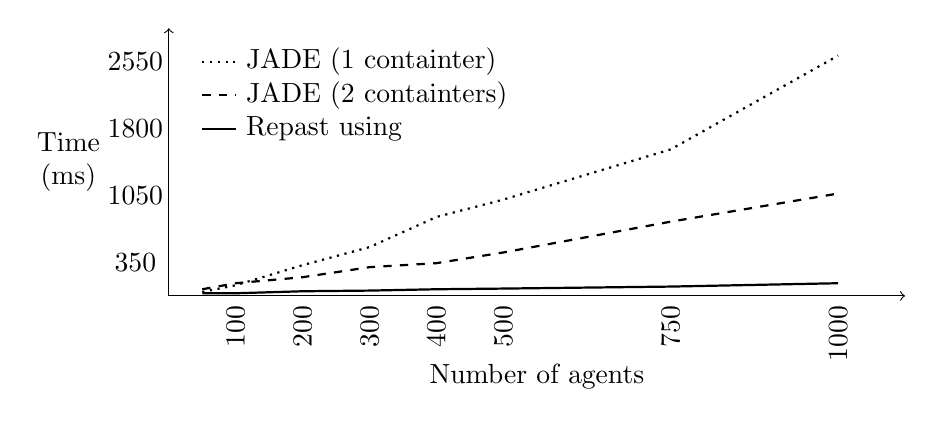
\begin{tikzpicture}[scale=0.85]

		% horizontal axis
		\draw[->] (0,0) -- (11,0);
		\draw (5.5,-1.2) node[align=center] {Number of agents}; %label

		
		% labels
		\draw	%(0.5,0) node[rotate=90, anchor=east] {50}
				(1.0,0) node[rotate=90, anchor=east] {100}
				(2.0,0) node[rotate=90, anchor=east] {200}
				(3.0,0) node[rotate=90, anchor=east] {300}
				(4.0,0) node[rotate=90, anchor=east] {400}
				(5.0,0) node[rotate=90, anchor=east] {500}
				(7.5,0) node[rotate=90, anchor=east] {750}
				(10.,0) node[rotate=90, anchor=east] {1000};

		\draw	(-0.5,0.5) node[anchor=center] {350}
				(-0.5,1.5) node[anchor=center] {1050}
				(-0.5,2.5) node[anchor=center] {1800}
				(-0.5,3.5) node[anchor=center] {2550};
		% vertical axis
		\draw[->] (0,0) -- (0,4);
		\draw (-1.5,2) node[align=center] {Time\\(ms)}; %label
		%\draw (-1.5,1.6) node[align=center] {(ms)}; %label

		%% Data %%
		% JADE 2 containers
		\draw[thick,dashed] (0.5,3.0) --
			(1,3.0) node[anchor=west, pos=1.0] {JADE (2 containters)}; %subtitle
		\draw[thick,dashed] (0.5, 0.10) --
					(1.0, 0.19) --
					(2.0, 0.28) --
					(3.0, 0.43) --
					(4.0, 0.49) --
					(5.0, 0.65) --
					(7.5, 1.11) --
					(10., 1.53);
		% JADE 1 containers
		\draw[thick,dotted] (0.5,3.5) --
			(1,3.5) node[anchor=west, pos=1.0] {JADE (1 containter)}; %subtitle
		\draw[thick,dotted] (0.5, 0.06) --
					(1.0, 0.16) --
					(2.0, 0.46) --
					(3.0, 0.73) --
					(4.0, 1.18) --
					(5.0, 1.44) --
					(7.5, 2.19) --
					(10., 3.59);
		% Repast
		\draw[thick] (0.5,2.5) --
			(1,2.5) node[anchor=west, pos=1.0] {Repast using \apiname{}}; %subtitle
		\draw[thick] (0.5, 0.04) --
					(1.0, 0.04) --
					(2.0, 0.07) --
					(3.0, 0.08) --
					(4.0, 0.10) --
					(5.0, 0.11) --
					(7.5, 0.14) --
					(10., 0.19);


	\end{tikzpicture}
	\caption[Execution performance in a simple contract net]
	{Average execution time of each framework in the different experiments.}
	\label{fig:performance}
\end{figure}